\documentclass[12pt, twoside]{article}
\usepackage[francais]{babel}
\usepackage[T1]{fontenc}
\usepackage[latin1]{inputenc}
\usepackage[left=7mm, right=7mm, top=7mm, bottom=7mm]{geometry}
\usepackage{float}
\usepackage{graphicx}
\usepackage{array}
\usepackage{multirow}
\usepackage{amsmath,amssymb,mathrsfs} 
\usepackage{soul}
\usepackage{textcomp}
\usepackage{eurosym}
\usepackage{lscape} 
 \usepackage{variations}
\usepackage{tabvar}
 
\pagestyle{empty} 

\title{\ul{\textbf{Nombres d�cimaux et op�rations}}}
\date{} 

\begin{document}
\maketitle


\section{Ecriture en lettres}


\ul{Exemple}: trente-six unit�s et cinquante-quatre centi�mes

\enskip

\fbox{
\begin{minipage}{19cm}
\ul{Orthographe}: Au pluriel, les mots servant � �crire les nombres sont en
g�n�ral invariables. Exceptions:


\begin{itemize}
  \item [$\bullet$] Les mots \textbf{cent} et \textbf{vingt} prennent un ``s''
  au pluriel lorsqu'ils ne sont pas suivis par un autre nombre.
  \item [$\bullet$] Les mots \textbf{million} et \textbf{milliard} sont des
  noms qui s'accordent au pluriel.
\end{itemize}
\end{minipage}}


\bigskip 

\ul{Exemples}: Les quatre fr�res \qquad \qquad \qquad \quad Cinq cent douze
mille habitants

Cinq mille quatre cents m�tres \qquad \qquad \qquad Sept millions deux cent
mille habitants

\bigskip



\fbox{
\begin{minipage}{19cm}
\ul{Orthographe}: Pour �crire en toutes lettres un nombre inf�rieur � 100, on
place un \textbf{trait d'union} entre les mots. Il est parfois remplac� par le
mot \textbf{et}.
\end{minipage}}


\bigskip

\ul{Exemples}: Soixante-douze heures \qquad \qquad \qquad Quarante et un
voleurs

\bigskip


\textit{Faire les exercices 1 et 2}

\section{Z�ros inutiles}


On peut supprimer ou ajouter des 0 � droite de la partie d�cimale d'un nombre.

\enskip

\ul{Exemples}: 5,300=5,3 \qquad \qquad 82,9=82,90 \qquad \qquad 12=12,0

Par contre: 0,82 $\neq$ 82  \qquad \qquad 920,3 $\neq$ 92,3


\enskip

\ul{Propri�t�}: Tout nombre entier est un nombre d�cimal dont la partie
d�cimale est nulle.

\enskip

\ul{Exemple}: Le nombre entier 49 est un nombre d�cimal: 49=49,0=49,00 \ldots


\bigskip

\textit{Faire les exercices 3, 4 et 5}



\section{Additions et soustractions}



Pour effectuer une addition ou une soustraction en colonne, on �crit les unit�s
sous les unit�s et on rajoute �ventuellement des z�ros inutiles.

\enskip

\ul{Exemples}: Poser et calculer: 


\begin{center}

\begin{tabular}{cc}
285,64 + 73,2 \qquad \qquad \qquad \qquad & \qquad \qquad \qquad \qquad 
78,38 - 21,943
\end{tabular}
\end{center}



\bigskip

\bigskip

\bigskip

\bigskip


\bigskip


\textit{Faire l'exercice 6}


\section{Multiplications}

\begin{center}
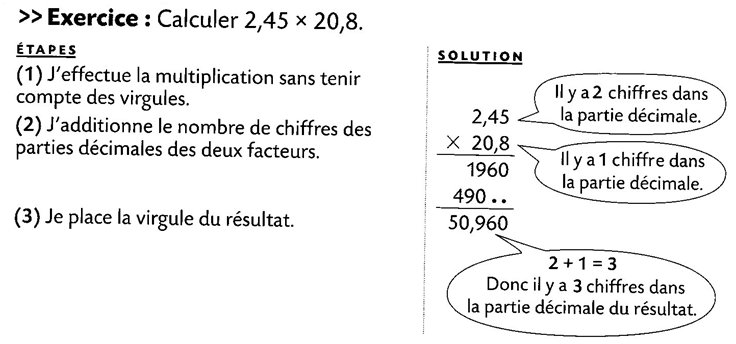
\includegraphics[width=11cm]{images/methode_produit.jpg}
\end{center}
  

\enskip

\ul{Exemple}: Poser et calculer $3,518 \times 2,4$

\bigskip

\bigskip

\bigskip


\bigskip

\bigskip



\textit{Faire l'exercice 7}


\section{Divisions}

\begin{tabular}{cc}
\begin{minipage}{5cm}
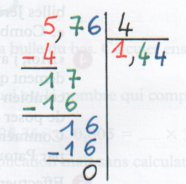
\includegraphics[width=4cm]{images/division.jpg}
\end{minipage}
&
\begin{minipage}{13cm}
\begin{enumerate}
  \item Dans 5, combien de fois je peux mettre 4? 1 fois. J'�cris 1 au quotient.
  \item 4 x 1 = 4, j'�cris la soustraction dans le calcul, il reste 1.
  \item J'abaisse le chiffre suivant ``7''. D�s que je d�passe la virgule, je
  la rajoute imm�diatement au quotient.
  \item Je continue: ``dans 17 combien de fois 4?'' 4 fois.
  
  
   J'�cris 4 au
  quotient.
  \item 4 x 4 = 16, j'�cris la soustraction, il reste 1.
  \item J'abaisse le chiffre suivant \ldots
\end{enumerate}
\end{minipage}
\end{tabular}

\bigskip

\bigskip

\textit{Faire l'exercice 8}

\end{document}
